\Tr
\onecolumn
IC170922A track parameters: $\alpha=77.43^{\circ +0.95}_{~-0.65} \quad \delta=5.72^{\circ +0.50}_{~-0.30} \quad E_{\nu}=290$ TeV
\begin{center}
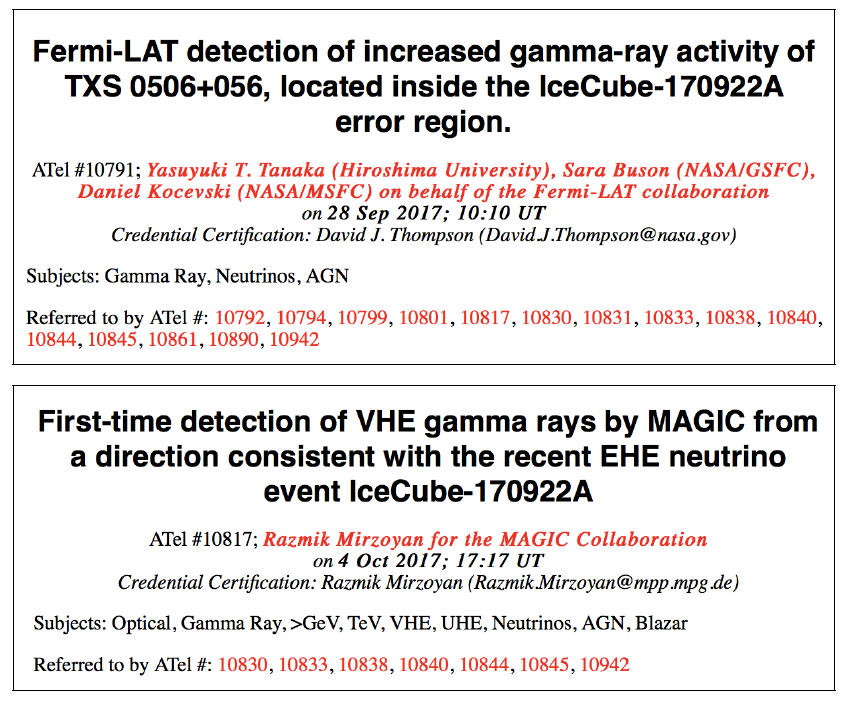
\includegraphics[keepaspectratio,height=14cm]{IC170922A}
\end{center}

\Tr
\twocolumn[\begin{center}{\blue The IC170922A area}\end{center}]
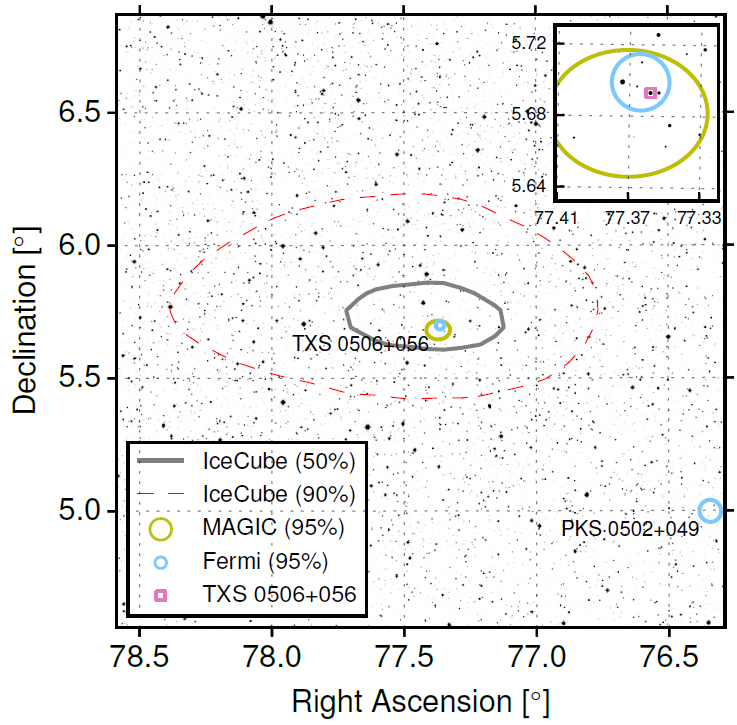
\includegraphics[keepaspectratio,width=13.5cm]{IC170922A-area}

\newpage

\begin{itemize}
\item Many radio and X-ray sources 
\item[] Most lack the needed energetics
\item Only 2 candidates remain\\
      {\large [Padovani et al. MNRAS 12-jul-2018]}
\item[$\ast$] TXS 0506+056 (BL Lac $z=0.3365$)
\item[] $D_{phys}=1.37$Gpc ($\sim$4.5 Gly)
\item[$\ast$] PKS 0502+049 (FSRQ $z=0.954$)
\item[] $D_{phys}=3.29$Gpc ($\sim$11 Gly)
\item Only TXS satisfies $\nu$ constraints\\
      (spatial, temporal and energetic)
\item[] PKS is $1.22^{\circ}$ away from TXS
\end{itemize}

\Tr
\onecolumn
\begin{center}
{\blue Addressing a random flaring Blazar coincidence with IC170922A}
\end{center}
%
\begin{itemize}
\item Consider the 90\% uncertainty patch around IC170922A and "Play darts"
\item[] $\rightarrow p(r) \sim 0.001/4\pi$ to randomly obtain a Blazar from an isotropic population
\item The Fermi 3LAC catalogue: 660 BL Lac and 440 FSRQ $\rightarrow$ Total: 1144 Blazars
\item[] $\sim 3$\% of Blazars similar to TXS are found to be flaring 
\item[] $\rightarrow p(r) \sim 3 \cdot 10^{-3}$ to randomly obtain a flaring Blazar from the sample
\item Using the temporal correlation with the flare
\item[$\ast$] Needs detailed information the TXS lightcurve $\rightarrow$ Likelihood analysis
\item[] Flaring activity observed on timescales of 40-180 days
\item IceCube observed 24 EHE neutrinos in 7 years $\rightarrow$ rate $\sim 0.01$ per day
\item[] Random EHE $\nu$ within flare period $\rightarrow$ Poisson distr. with mean $0.4 \le \mu \le 1.8$
\item[] Probability to find at least 1 EHE $\nu$ in flare period: $0.33 \le p(n \ge 1|\mu) \le 0.83$
\item Probability for a random coincidence: $10^{-3} \le p(r) \le 2.5 \cdot 10^{-3}~(\le 3\sigma)$
\end{itemize}

\Tr
\onecolumn
\begin{center}
{\blue The IceCube 9.5 years archival dataset}\\[3mm]
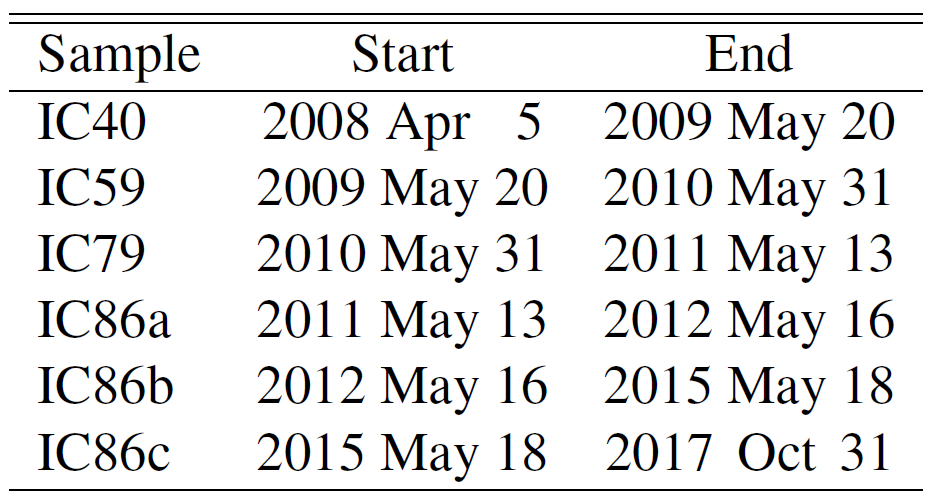
\includegraphics[keepaspectratio,height=12cm]{IC-archival-dataset}\\[3mm]
{\red Note : IC170922A happened in the data period IC86c}
\end{center}

\Tr
\onecolumn
\begin{center}
{\blue The IceCube archival analysis result}
\end{center}
%
\begin{itemize}
\item Use the TXS 0506+056 location for evaluation
\item Use unbinned likelihood with a Gaussian spatial pdf and $\Phi \cdot E^{-\gamma}$ energy pdf
\item Use a Gauss c.q. Box time window $T_{W}$ around a central time $T_{0}$
\item[] $\rightarrow$ Search for event clustering with Spatial*Energy*Time weights
\item Use randomized data to represent background and determine the significance
\item[] $\rightarrow$ Find ($\Phi,\gamma,T_{0},T_{W}$) that maximizes the likelihood ratio
\end{itemize}
%
\begin{center}
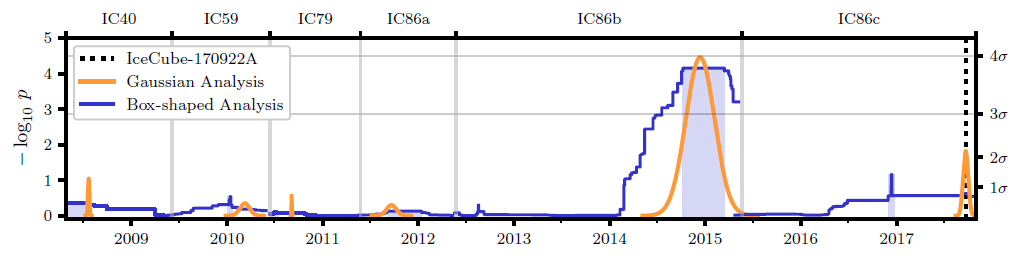
\includegraphics[keepaspectratio,width=26cm]{txs-time-dependent}
\end{center}


\Tr
\onecolumn
\begin{center}
{\blue Spatial*Energy weights for the IceCube archival IC86b data}\\[3mm]
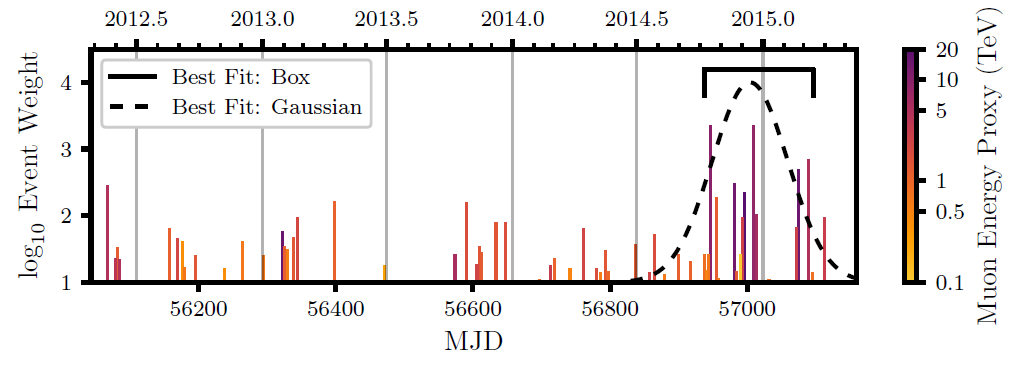
\includegraphics[keepaspectratio,width=24cm]{txs-time-dependent-IC86b}
\end{center}
%
\begin{itemize}
\item Gaussian time window: $T_{0}=$13-dec-2014 $\pm$ 21 days $T_{W}=110^{+35}_{-24}$days
\item Excess of $13 \pm 5$ events above atmospheric background 
\item Best spectral fits: $\int \Phi dt=2.1^{+0.9}_{-0.7} \cdot 10^{-4}$ TeV cm$^{-2}$ at 100 TeV $\quad \gamma=2.1 \pm 0.2$
\item Box time window: $T_{0}=$26-dec-2014 $T_{W}=$158 days and similar spectrum
\end{itemize}

\Tr
\onecolumn
\begin{center}
{\blue Fermi lightcurve for IC170922A}\\[3mm]
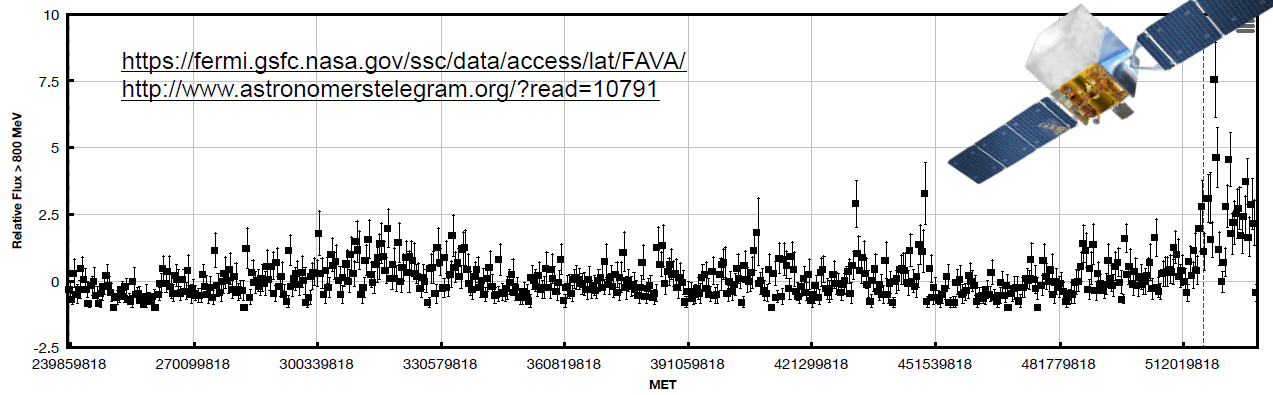
\includegraphics[keepaspectratio,width=25cm]{IC170922A-Fermi}\\
{\large [Credit M. Kowalski SuGAR2018]}
\end{center}

\Tr
\onecolumn
\begin{center}
{\blue The TXS 0506+056 Multi-wavelength lightcurves}\\[3mm]
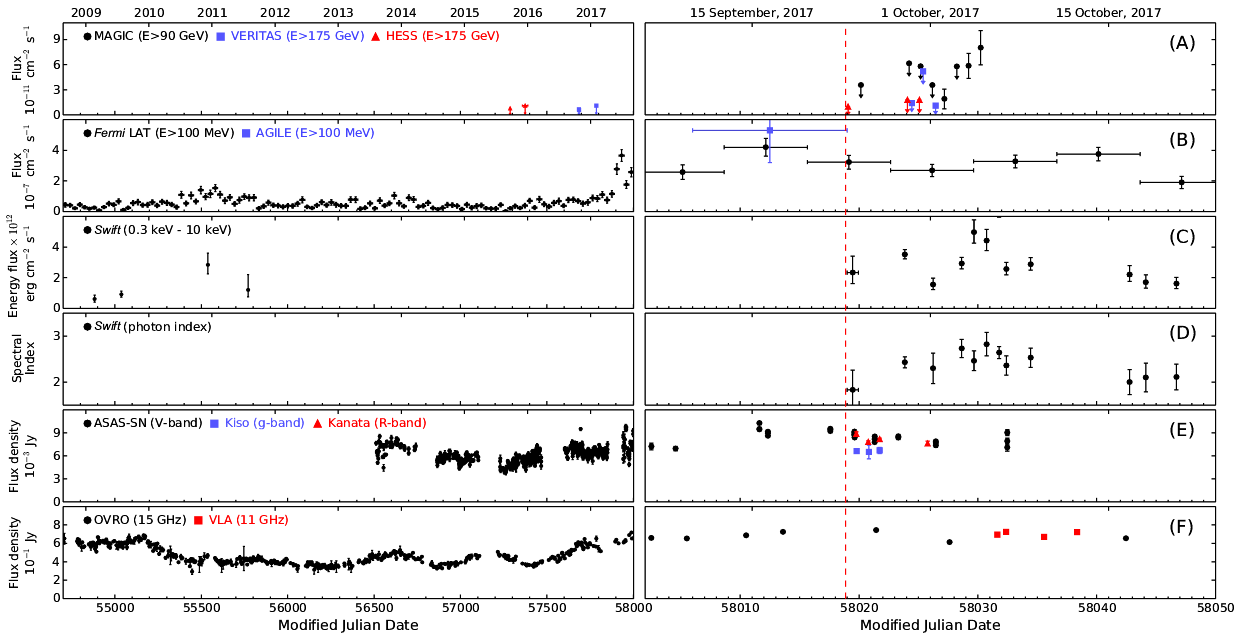
\includegraphics[keepaspectratio,width=26cm]{txs-mw-lightcurves}
\end{center}

\Tr
\twocolumn
\begin{itemize}
\item Fermi EGB observations
\item[] {\blue $\sim$85\% of diffuse $\gamma$'s from Blazars}
\item IceCube observations {\large [ApJ 835 (2017) 45]}
\item[] {\blue Cosmic $\nu$'s NOT from Fermi Blazars}
\item Take EGB NON-Blazar component
\item[] $\rightarrow$ {\blue Prediction for $\nu$ flux}
\end{itemize}
%
\begin{itemize}
\item[$\ast$] {\red $\nu$ flux underestimated}
\item[] Fermi and IceCube data tension
\item {\red Cosmic $\nu$'s from obscured sources ?}\\
      {\large [PRD 94 (2016) 103007]}
\item Dust may provide a "CR beam dump"
\item[] $\rightarrow$ Neutrino factory
\end{itemize}

\newpage
%
\begin{center}
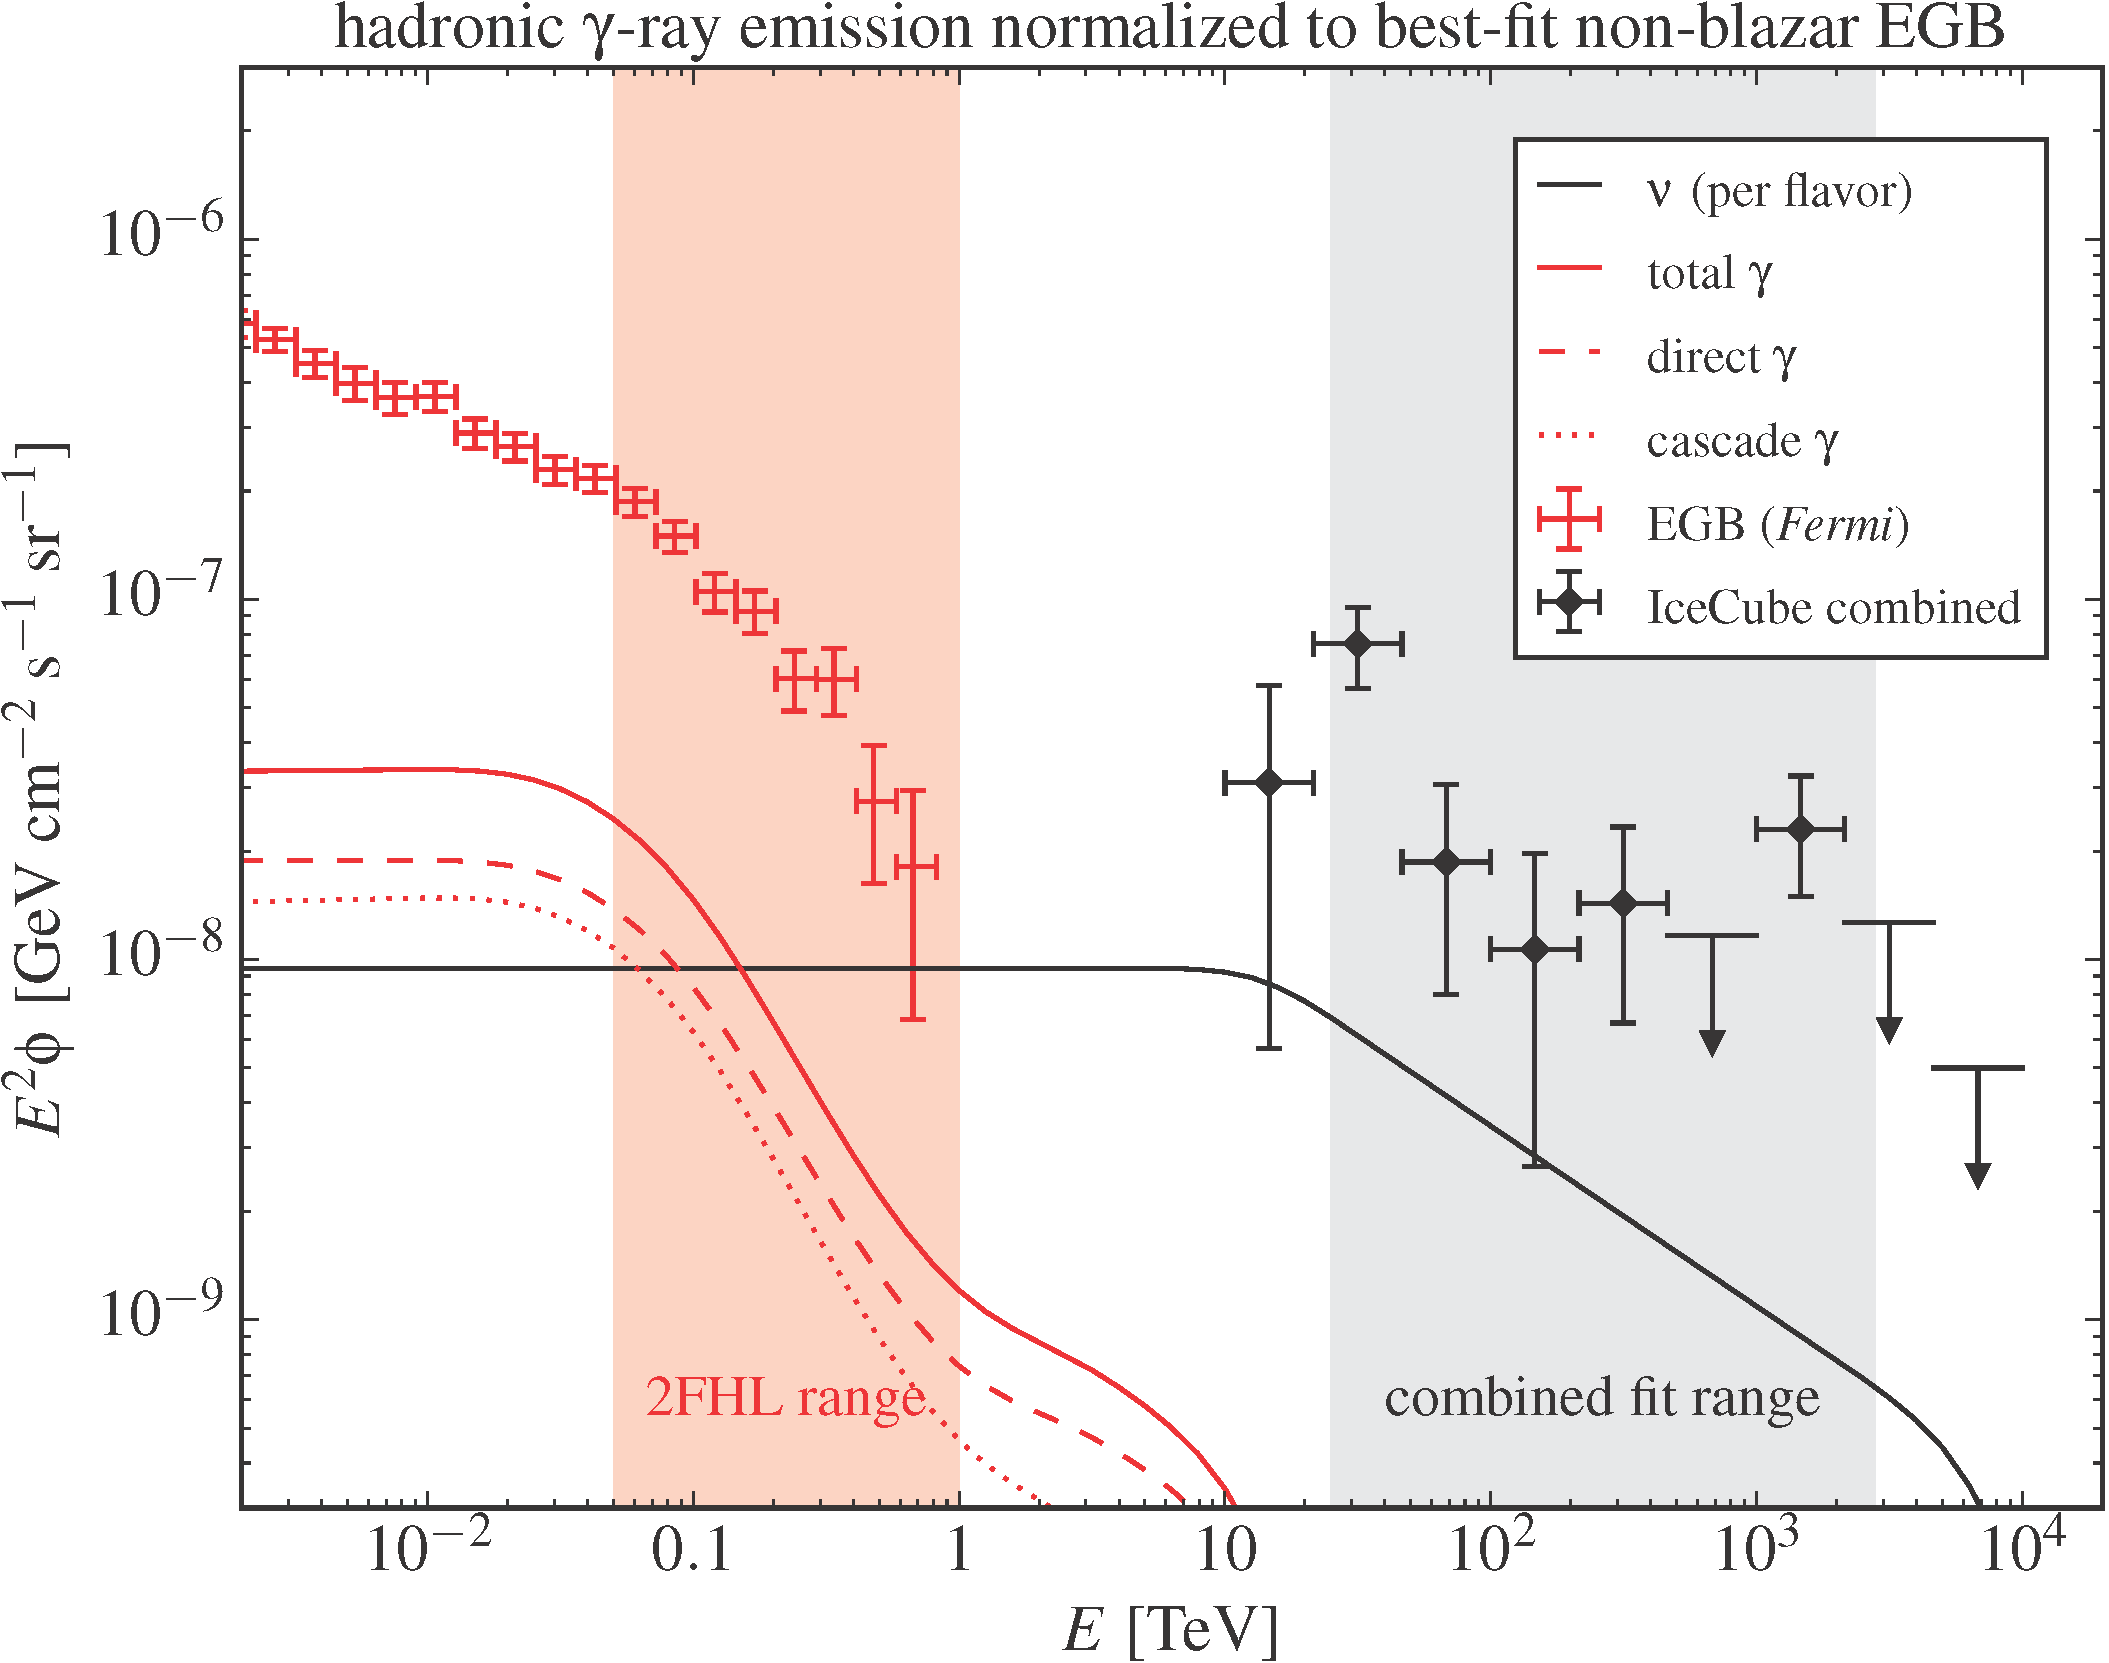
\includegraphics[keepaspectratio,width=13cm]{Fermi-IC}\\
{\large [arXiv:1511.00688]}
\end{center}
\begin{itemize}
\item[] (2FHL: 2nd Fermi Hard Source List)
\end{itemize}
